\Variant{27.12.2025}
\QQ{1}{$88$, $95$, $96$ va $a$ sonlarining örta arifmetigi $94$ ga teng bölsa, $a$ ning qiymatini toping.
\Opts{$105$}{$85$}{$97$}{$75$}}
\QQ{2}{Quyidagilardan neçtasi irratsional son:\par
1) $\pi+\sqrt{10}$; \ 2) $\dfrac{22}7$; \ 3) $\sqrt[3]{2-\sqrt5}+\sqrt[3]{2+\sqrt5}$;\par
4) $3{,}2(525)$; \ 5) $\sqrt{4-2\sqrt3}+\sqrt{4+2\sqrt3}$
\Opts{$2$}{$3$}{$4$}{barçasi}}
\QQ{3}{Anvar Şerzodga qaraganda $5$ kun köp işladi, Jasur esa Şerzodga qaraganda $4$ kun kam işladi. Agar uççalasi işni $3$ kunda bajarsa, Şerzod bir özi işni neça kunda bajaradi?
\Opts{$10$}{$6$}{$15$}{$11$}}
\QQ{4}{Mahsulotning dastlabki narxi $400\,000$ söm edi. Avval narx $30\%$ ga kamaytirildi, şundan söng narx $10\%$ ga oşirildi. Mahsulotning oxirgi narxini toping.
\Opts{$300\,000$}{$280\,000$}{$308\,000$}{$380\,000$}}
\QQ{5}{Hisoblang:
\[\frac{1^3+2^3+\dots+9^3}{2025}\]
\Opts{$1$}{$2$}{$3$}{$4$}}
\QQ{6}{Hisoblang:
\[\sqrt{\frac{11^4+100^4+111^4}2}\]
\Opts{$11223$}{$11221$}{$11022$}{$11233$}}
\QQ{7}{Agar $\left(2x^3-x^2+1\right)^5\cdot(x-2)^3$ köpaytmani soddalaştirgandan keyin $x^2$ li hadining oldidagi koeffitsiyentni toping.
\Opts{$52$}{$-40$}{$34$}{$12$}}
\QQ{8}{Arifmetik progressiyada $a_2+a_4=16$ va $a_1\cdot a_5=28$ bölsa, $a_2$ ni toping.
\Opts{$4$ yoki $10$}{$5$ yoki $11$}{$7$ yoki $12$}{$6$ yoki $15$}}
\QQ{9}{Ösuvçi geometrik progressiyada $b_1+b_2+b_3=91$ va $b_3-b_2=42$ bölsa, $S_2$ ni toping.
\Opts{$30$}{$29$}{$28$}{$27$}}
\QQ{10}{Agar $x+\dfrac1x=6$ bölsa, $\dfrac{x^4+1}{4x^2}$ ning qiymatini toping.
\Opts{$6\dfrac14$}{$8\dfrac12$}{$9\dfrac12$}{$9\dfrac14$}}
\QQ{11}{Soddalaştiring:
\[\sqrt[6]{2x\left(7+3\sqrt5\right)}\cdot\sqrt[3]{\sqrt{5x}-3\sqrt x}\]
\Opts{$2\sqrt[3]{2x}$}{$\sqrt[3]{4x}$}{$-\sqrt[3]{4x}$}{$\sqrt[3]{2x}$}}
\QQ{12}{Soddalaştiring:
\[\frac{2\sin20^\circ+\sin40^\circ}{2\sin20^\circ-\sin40^\circ}\]
\Opts{$\tg^210^\circ$}{$\cos^210^\circ$}{$\ctg^210^\circ$}{$\sin^210^\circ$}}
\QQ{13}{Quyidagi tenglamalar sistemasi $[-2\pi;\,2\pi]$ oraliqda neçta ildizga ega?
\[\begin{cases}x+y=\dfrac\pi3,\\[4pt] \sin x\cdot\sin y=\dfrac14\end{cases}\]
\Opts{$1$}{$2$}{$3$}{$4$}}
\QQ{14}{$8+2^x\cdot x+2^{3-x}=x$ tenglamaning neçta haqiqiy ildizi bor?
\Opts{$2$}{$1$}{$0$}{$3$}}
\QQ{15}{Tenglamaning ildizlari yiğindisini toping:
\[\log_2^2x+(x-1)\log_2x=6-2x\]
\Opts{$1{,}25$}{$1{,}75$}{$2{,}25$}{$2$}}
\QQ{16}{Quyidagi tenglamalar sistemasi berilgan bölsa, $x+y$ ning qiymatini toping.
\[\begin{cases}3x-y=16,\\ x+2y=17\end{cases}\]
\Opts{$10$}{$12$}{$15$}{$11$}}
\QQ{17}{$x^3-(x+1)^2=2001$ tenglama neçta yeçimga ega?
\Opts{$\varnothing$}{$1$}{$2$}{$3$}}
\QQ{18}{Tengsizlikni qanoatlantiruvçi butun sonlar neçta?
\[x^2-8x-\frac{3x-12}{|x-4|}+18\le0\]
\Opts{$1$}{$0$}{$3$}{$4$}}
\QQ{19}{Tengsizlikni neçta butun son qanoatlantiradi?
\[\sqrt{x-8\sqrt{8+x}+24}-\frac{16+x}{2\sqrt{8+x}-10}<0\]
\Opts{$10$}{$11$}{$230$}{$231$}}
\QQ{20}{$f(x)=2x^2+(a-10)x+6$ funksiya nollari $x_1$ va $12x_1$ bölsa, şunday $a$ larning yiğindisini toping.
\Opts{$20$}{$23$}{$-3$}{$18$}}
\QQ{21}{Aniq integralni hisoblang:
\[\int_0^1\frac{6x^2}{\left(4-x^3\right)^2}\,dx\]
\Opts{$\dfrac1{12}$}{$-\dfrac16$}{$\dfrac16$}{$-\dfrac1{12}$}}
\QQ{22}{$y=\sqrt{\dfrac72x^2-7}$ funksiya grafigiga ötkazilgan urinma $y=ax+b$ bölsin. Agar $y=-\dfrac12x+3$ töğri çiziq grafigi $y=ax+b$ funksiya bilan özaro perpendikulyar bölsa, $a+b$ ning qiymatini toping.
\Opts{$1$}{$2$}{$-1$}{$3$}}
\QQ{23}{Aylanada özaro teng va perpendikulyar vatarlar bölib, aylanadagi $A$ nuqtada umumiy uçiga ega. Agar aylana markazidan vatargaça bölgan eng qisqa masofa $8$ sm bölsa, vatar uzunligini toping.
\Opts{$16$}{$16\sqrt2$}{$20$}{$26$}}
\QQ{24}{Agar $f(x)=\dfrac3{\sqrt{1+x}}$ bölsa, $f^{-1}(2)$ ning qiymatini toping. ($f^{-1}(x)$ — $f(x)$ funksiyaning teskari funksiyasi.)
\Opts{$\dfrac14$}{$2\dfrac14$}{$1\dfrac14$}{$2\dfrac34$}}
\QQ{25}{Rasmda berilgan maʼlumotlar asosida $x$ ning uzunligini toping.
\qfig{\begin{tikzpicture}[scale=0.85,font=\scriptsize]
\coordinate (O) at (0,0);
\coordinate (P0) at (-6,0); \coordinate (P1) at (-4.5,2.598); \coordinate (P2) at (-2.25,3.897); \coordinate (P3) at (0,3.897); \coordinate (P4) at (1.688,2.923); \coordinate (P5) at (2.531,1.461); \coordinate (P6) at (2.531,0);
\draw (O)--(P0)--(P1)--(P2)--(P3)--(P4)--(P5)--(P6)--cycle;
\foreach \p in {P1,P2,P3,P4,P5} \draw (O)--(\p);
\foreach \p/\q in {P1/P0,P2/P1,P3/P2,P4/P3,P5/P4,P6/P5} \draw ($(\p)!0.22cm!(\q)$) -- ($($(\p)!0.22cm!(\q)$)!1!-90:(\p)$) -- ($(\p)!0.22cm!(O)$);
\foreach \k in {0,...,5} {\draw ({180-30*\k}:0.55) arc ({180-30*\k}:{150-30*\k}:0.55); \node at ({165-30*\k}:0.95) {$30^\circ$};}
\node[below] at (-3,0) {\small$64$}; \node[below] at (1.27,0) {\small$x$};
\end{tikzpicture}}
\Opts{$9\sqrt3$}{$27$}{$18\sqrt3$}{$18$}}
\QQ{26}{$ABC$ uçburçakning $BC$ tomonidan $D$ nuqta olingan. $AD$ kesma $ABC$ uçburçakni ikkita $ABD$ va $ADC$ uçburçaklarga ajratadi. $ABD$ va $ADC$ uçburçaklarga içki çizilgan aylanalar $AD$ kesmaga mos ravişda $E$ va $F$ nuqtalarda urinadi. Agar $AB=5$, $AC=7$, $BD=5$ va $DC=3$ bölsa, $EF$ kesma uzunligini toping.
\qfig{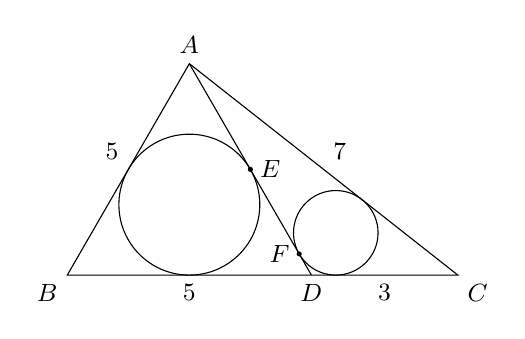
\begin{tikzpicture}[scale=0.62,font=\small]
\coordinate (B) at (0,0); \coordinate (C) at (8,0); \coordinate (A) at (2.5,4.330); \coordinate (D) at (5,0);
\coordinate (E) at (3.75,2.165); \coordinate (F) at (4.75,0.433);
\draw (A)--(B)--(C)--cycle; \draw (A)--(D);
\draw (2.5,1.443) circle (1.443); \draw (5.5,0.866) circle (0.866);
\fill (E) circle (1.5pt); \fill (F) circle (1.5pt);
\node[above] at (A) {$A$}; \node[below left] at (B) {$B$}; \node[below right] at (C) {$C$}; \node[below] at (D) {$D$};
\node[right] at (E) {$E$}; \node[left] at (F) {$F$};
\node[above left] at (1.25,2.165) {$5$}; \node[above right] at (5.25,2.165) {$7$}; \node[below] at (2.5,0) {$5$}; \node[below] at (6.5,0) {$3$};
\end{tikzpicture}}
\Opts{$1$}{$2$}{$3$}{$1{,}5$}}
\QQ{27}{$ABCD$ trapetsiyaning $AB$ va $CD$ asoslari mos ravişda $4$ va $12$ ga teng. Trapetsiyaning $AB$ va $CD$ asoslariga parallel $EF$ kesma ötkazilgan. $EF$ kesma $BD$ diagonal bilan $O$ nuqtada kesişadi. Agar $EOD$ va $BOF$ uçburçaklar yuzlari teng bölsa, $EF$ kesma uzunligini toping.
\qfig{\begin{tikzpicture}[scale=0.42,font=\small]
\coordinate (D) at (0,0); \coordinate (C) at (12,0); \coordinate (A) at (3.2,7); \coordinate (B) at (7.2,7);
\coordinate (E) at (2.029,4.438); \coordinate (F) at (8.958,4.438); \coordinate (O) at (4.565,4.438);
\fill[qfill] (E)--(O)--(D)--cycle; \fill[qfill] (B)--(O)--(F)--cycle;
\draw (A)--(B)--(C)--(D)--cycle; \draw (E)--(F); \draw (B)--(D);
\node[above left] at (A) {$A$}; \node[above right] at (B) {$B$}; \node[below right] at (C) {$C$}; \node[below left] at (D) {$D$};
\node[left] at (E) {$E$}; \node[right] at (F) {$F$}; \node[below right] at (O) {$O$};
\node[above] at (5.2,7) {$4$}; \node[below] at (6,0) {$12$};
\end{tikzpicture}}
\Opts{$4\sqrt3$}{$6$}{$10\sqrt3$}{$5$}}
\QQ{28}{$ABCDE$ muntazam beşburçak berilgan. $DE$ tomoni $E$ tomonga davom ettirilib, unda $O$ nuqta olindi, $DO=8$. $G$ nuqta $AB$ tomonning örtasi bölib, $OG$ kesma $EA$ tomonni $F$ nuqtada kesib ötadi va $\angle OFE=45^\circ$. $H$ nuqta $BC$ tomonning örtasi. $EH$ ning uzunligini toping.
\qfig{\begin{tikzpicture}[scale=1.25,font=\small]
\coordinate (D) at (0.000,1.500); \coordinate (C) at (1.427,0.464); \coordinate (B) at (0.882,-1.214); \coordinate (A) at (-0.882,-1.214); \coordinate (E) at (-1.427,0.464); \coordinate (G) at (0.000,-1.214); \coordinate (H) at (1.154,-0.375); \coordinate (O) at (-2.195,-0.095); \coordinate (F) at (-1.057,-0.675);
\draw (A)--(B)--(C)--(D)--(E)--cycle; \draw (D)--(O)--(G); \draw (D)--(G); \draw (E)--(H);
\draw ($(D)!0.3cm!(E)$) arc (216:270:0.3cm); \node at ($(D)+(250:0.55)$) {\scriptsize$54^\circ$};
\node[below] at (A) {$A$}; \node[below] at (B) {$B$}; \node[right] at (C) {$C$}; \node[above] at (D) {$D$}; \node[above left] at (E) {$E$};
\node[below] at (G) {$G$}; \node[right] at (H) {$H$}; \node[left] at (O) {$O$}; \node[below left] at (F) {$F$};
\node at ($(F)+(-25:0.33)$) {\scriptsize$45^\circ$};
\end{tikzpicture}}
\Opts{$8$}{$16$}{$8\sqrt2$}{$15$}}
\QQ{29}{Koordinatalar sistemasida $A(-5;\,4)$, $B(14;\,5)$, $C(3;\,-3)$ nuqtalar berilgan. Şu nuqtalarni tutaştirib $ABC$ uçburçak hosil qilindi. Koordinata boşidan $ABC$ uçburçakning oğirlik markazigaça bölgan masofani toping.
\qfig{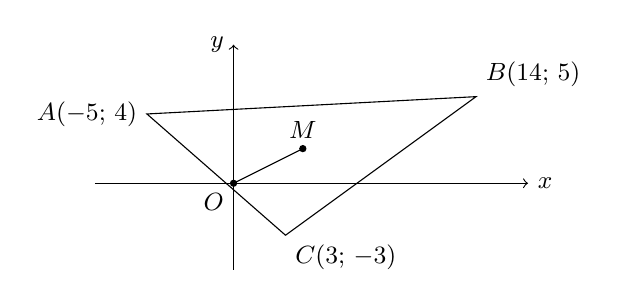
\begin{tikzpicture}[scale=0.22,font=\small]
\draw[->] (-8,0)--(17,0) node[right] {$x$}; \draw[->] (0,-5)--(0,8) node[left] {$y$};
\draw (-5,4)--(14,5)--(3,-3)--cycle; \draw (0,0)--(4,2);
\fill (0,0) circle (6pt); \fill (4,2) circle (6pt);
\node[left] at (-5,4) {$A(-5;\,4)$}; \node[above right] at (14,5) {$B(14;\,5)$}; \node[below right] at (3,-3) {$C(3;\,-3)$};
\node[above] at (4,2) {$M$}; \node[below left] at (0,0) {$O$};
\end{tikzpicture}}
\Opts{$\sqrt5$}{$1$}{$2\sqrt5$}{$0{,}5$}}
\QQ{30}{$\alpha$ va $\beta$ tekisliklar özaro parallel. $\alpha$ tekislikda $A$, $B$ nuqtalar olingan. $A$ va $B$ nuqtalardan $\beta$ tekislikka $AC$ va $BD$ oğmalar tuşirilgan. Agar $AC=37$, $BD=125$ va $AC$ oğma proyeksiyasi $12$ ga teng bölsa, $BD$ ning $\beta$ tekislikdagi proyeksiyasini toping.
\Opts{$120$}{$144$}{$140$}{$100$}}
\QQ{31}{Agar $A=\{a;\,b;\,c;\,d\}$ va $B=\{a;\,b;\,m;\,n;\,k\}$ bölsa, $A\cup B$ ning qism töplamlar sonini toping.
\Opts{$7$}{$64$}{$128$}{$8$}}
\QQ{32}{Barça raqamlari toq raqamlardan iborat bölgan uç xonali sonlar $n$ ta, barça raqamlari juft raqamlardan iborat bölgan tört xonali sonlar $m$ ta bölsa, $\dfrac nm$ ning qiymatini toping.
\Opts{$\dfrac12$}{$\dfrac23$}{$\dfrac34$}{$\dfrac14$}}
\QQ{33}{\Moslash{$ABCDA_1B_1C_1D_1$ kubga markazi $O$ nuqtada bölgan şar içki çizilgan bölib, şar kubning uçta $ABCD$, $AA_1B_1B$ va $BB_1C_1C$ yoqlariga va $DD_1$ qirrasiga urinadi. Kubning qirrasi $\sqrt2$ ga teng.
\par\centering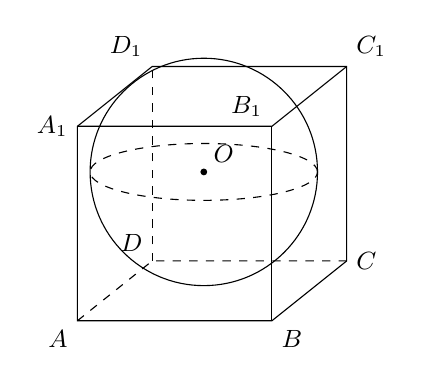
\begin{tikzpicture}[scale=0.95,font=\small]
\coordinate (A) at (0,0); \coordinate (B) at (2.6,0); \coordinate (C) at (3.6,0.8); \coordinate (D) at (1,0.8);
\coordinate (A1) at (0,2.6); \coordinate (B1) at (2.6,2.6); \coordinate (C1) at (3.6,3.4); \coordinate (D1) at (1,3.4);
\coordinate (O) at (1.69,1.99);
\draw[dashed] (A)--(D)--(C); \draw[dashed] (D)--(D1);
\draw (O) circle (1.52); \draw[dashed] (O) ellipse (1.52 and 0.38);
\draw (A)--(B)--(C)--(C1)--(D1)--(A1)--cycle; \draw (A1)--(B1)--(C1); \draw (B1)--(B);
\fill (O) circle (1.3pt); \node[above right] at (O) {$O$};
\node[below left] at (A) {$A$}; \node[below right] at (B) {$B$}; \node[right] at (C) {$C$}; \node[above left] at (D) {$D$};
\node[left] at (A1) {$A_1$}; \node[above left] at (B1) {$B_1$}; \node[above right] at (C1) {$C_1$}; \node[above left] at (D1) {$D_1$};
\end{tikzpicture}}{A) $\sqrt2-1$\par B) $2\sqrt2-2$\par C) $2+\sqrt2$\par D) $2-\sqrt2$\par E) $2\sqrt2-1$\par F) $4-2\sqrt2$}{Şarning radiusini toping.}{$O$ nuqtadan $AA_1D_1D$ yoqqaça bölgan eng qisqa masofani toping.}{$O$ nuqtadan $D$ nuqtagaça bölgan masofani toping.}}
\QQ{36}{Tenglamalar sistemasi berilgan:
\[\begin{cases}x^2+y^2=4-2ay-a^2,\\ y-x^2=0\end{cases}\]
\AB{Sistema bitta yeçimga ega böladigan $a$ ning butun qiymatlari yiğindisini toping.}{Sistema ikkita har xil yeçimga ega böladigan $a$ ning eng kiçik qiymatini toping.}}
\QQ{37}{Tenglamani yeçing:
\[\cos x+\cos2x+\cos3x=\sin x+\sin2x+\sin3x\]
\AB{Tenglamaning eng kiçik musbat yeçimini toping.}{$[-\pi;\,\pi]$ oraliqda tenglama neçta ildizga ega?}}
\QQ{38}{$f(x)=(x+a)^2+b$, $x\in[-a;\,\infty)$ berilgan. $g(x)$ funksiya $f(x)$ funksiyaning ösuvçi tarmoğiga teskari. $g(x)$ funksiya grafigi $(0;\,3)$ nuqtadan ötadi va $f(x)$ funksiyaning eng kiçik qiymati $-1$ ga teng.
\AB{$a+b$ ning qiymatini toping.}{$f(x)$ va $g(x)$ funksiyalar neçta nuqtada kesişadi?}}
\QQ{39}{Rasmda $f(x)=ax^2+bx+c$ parabola uçining koordinatasi $B(2;\,-3)$ berilgan.
\qfig{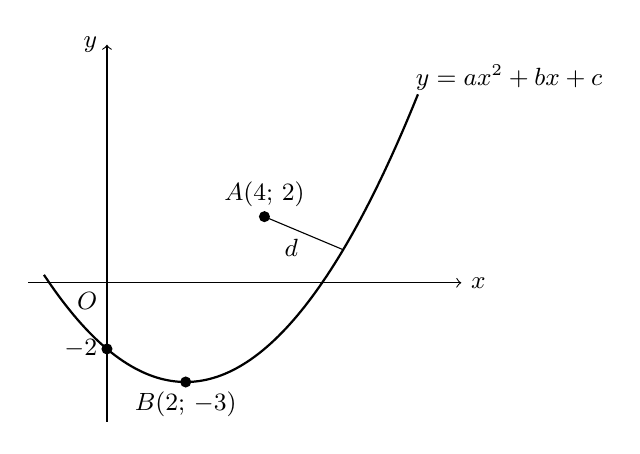
\begin{tikzpicture}[x=0.5cm,y=0.42cm,font=\small]
\draw[->] (-2,0)--(9,0) node[right] {$x$}; \draw[->] (0,-4.2)--(0,7.2) node[left] {$y$};
\draw[thick,domain=-1.6:7.9,samples=100] plot (\x,{\x*\x/4-\x-2});
\draw (4,2)--(6,1);
\fill (4,2) circle (2pt); \fill (2,-3) circle (2pt); \fill (0,-2) circle (2pt);
\node[above] at (4,2) {$A(4;\,2)$}; \node[below] at (2,-3) {$B(2;\,-3)$}; \node[left] at (0,-2) {$-2$};
\node[below left] at (5.1,1.6) {$d$}; \node[below left] at (0,0) {$O$};
\node[right] at (7.6,6.2) {$y=ax^2+bx+c$};
\end{tikzpicture}}
\AB{$\dfrac{ac}b$ ning qiymatini toping.}{$A(4;\,2)$ nuqtadan parabolagaça bölgan eng qisqa masofani toping.}}
\QQ{40}{Çizmada $y=ax^2+bx+c$ va $y=-|x+m|+n$ funksiya grafiklari tasvirlangan. Parabolaning uçi $(3;\,4)$ nuqtada.
\qfig{\begin{tikzpicture}[x=0.8cm,y=0.55cm,font=\small]
\fill[qfill] plot[domain=1:5,samples=80] (\x,{-(\x-1)*(\x-5)}) -- (3,2) -- cycle;
\draw[->] (-0.6,0)--(6.6,0) node[right] {$x$}; \draw[->] (0,-1.3)--(0,5) node[left] {$y$};
\draw[thick,domain=0.7:5.3,samples=100] plot (\x,{-(\x-1)*(\x-5)});
\draw[thick] (-0.1,-1.1)--(3,2)--(6.1,-1.1);
\draw[dashed] (3,0)--(3,4); \fill (3,4) circle (2pt); \node[above] at (3,4) {$(3;\,4)$};
\node[below left] at (0,0) {$O$}; \node[below right] at (1,0) {$1$}; \node[below left] at (5,0) {$5$};
\node[right] at (4.1,3.9) {$y=ax^2+bx+c$}; \node[below] at (3,-0.9) {$y=-|x+m|+n$};
\end{tikzpicture}}
\AB{$\dfrac{a+b-c}{n-m}$ ning qiymatini toping.}{Böyalgan soha yuzini toping.}}
\QQ{41}{$ABC$ uçburçakka içki aylana çizilgan. Bunda $D$ nuqta aylanaga uriniş nuqtasi va $AB=7$, $DC=3$, $\angle C=60^\circ$ bölsa:
\qfig{\begin{tikzpicture}[scale=0.62,font=\small]
\coordinate (A) at (0,0); \coordinate (C) at (8,0); \coordinate (B) at (5.5,4.330); \coordinate (D) at (5,0);
\draw (A)--(B)--(C)--cycle; \draw (5,1.732) circle (1.732); \fill (D) circle (1.6pt);
\draw ($(C)!0.6cm!(A)$) arc (180:120:0.6cm); \node at ($(C)+(150:0.95)$) {\scriptsize$60^\circ$};
\node[below left] at (A) {$A$}; \node[above] at (B) {$B$}; \node[below right] at (C) {$C$}; \node[below] at (D) {$D$};
\node[above left] at (2.75,2.165) {$7$}; \node[below] at (6.5,0) {$3$};
\end{tikzpicture}}
\AB{Aylana radiusini toping.}{$ABC$ uçburçakning yuzini toping.}}
\QQ{42}{$ABCD$ töğri törtburçakning $BC$ va $AD$ tomonlaridan mos ravişda $E$ va $F$ nuqtalar olingan. $AE$ va $BF$ çiziqlar $M$ nuqtada, $CF$ va $DE$ çiziqlar esa $N$ nuqtada kesişadi. $AMF$, $BME$, $CEN$, $DNF$ uçburçaklarning yuzalari mos ravişda $32$, $8$, $27$, $3$ ga teng bölsa,
\qfig{\begin{tikzpicture}[scale=0.42,font=\small]
\coordinate (A) at (0,0); \coordinate (D) at (12,0); \coordinate (C) at (12,10); \coordinate (B) at (0,10);
\coordinate (E) at (4.8,10); \coordinate (F) at (9.6,0); \coordinate (M) at (3.2,6.667); \coordinate (N) at (10.2,2.5);
\fill[qfill] (M)--(E)--(N)--(F)--cycle;
\draw (A)--(B)--(C)--(D)--cycle; \draw (A)--(E)--(D); \draw (B)--(F)--(C);
\node[below left] at (A) {$A$}; \node[above left] at (B) {$B$}; \node[above right] at (C) {$C$}; \node[below right] at (D) {$D$};
\node[above] at (E) {$E$}; \node[below] at (F) {$F$}; \node[left] at (M) {$M$}; \node[right] at (N) {$N$};
\node[draw,circle,inner sep=1pt] at (4.3,4.2) {\scriptsize$32$}; \node[draw,circle,inner sep=1pt] at (2.7,8.9) {\scriptsize$8$};
\node[draw,circle,inner sep=1pt] at (9.2,7.3) {\scriptsize$27$}; \node[draw,circle,inner sep=1pt] at (10.8,0.9) {\scriptsize$3$};
\end{tikzpicture}}
\AB{Böyalgan soha yuzini toping.}{$ABCD$ töğri törtburçak yuzini toping.}}
\QQ{43}{$ACDE$ töğri törtburçakka $B_1B_2B_3B_4B_5B_6$ muntazam oltiburçak rasmdagidek joylaştirilgan. $AB_1B_6$ uçburçakning yuzi $7$ ga, $EB_6B_5B_4$ törtburçakning yuzi $8$ ga teng bölsa:
\qfig{\begin{tikzpicture}[scale=0.4,font=\small]
\coordinate (E) at (0,0); \coordinate (D) at (10.926,0); \coordinate (C) at (10.926,9.885); \coordinate (A) at (0,9.885);
\coordinate (B6) at (0,5.365); \coordinate (B1) at (3.098,9.885); \coordinate (B2) at (8.561,9.462); \coordinate (B3) at (10.926,4.520); \coordinate (B4) at (7.828,0); \coordinate (B5) at (2.365,0.423);
\fill[qfill] (B6)--(B2)--(B3)--cycle;
\draw (A)--(C)--(D)--(E)--cycle; \draw (B1)--(B2)--(B3)--(B4)--(B5)--(B6)--cycle; \draw (B6)--(B2); \draw (B6)--(B3);
\node[above left] at (A) {$A$}; \node[above right] at (C) {$C$}; \node[below right] at (D) {$D$}; \node[below left] at (E) {$E$};
\node[above] at (B1) {$B_1$}; \node[above right] at (B2) {$B_2$}; \node[right] at (B3) {$B_3$}; \node[below] at (B4) {$B_4$}; \node[above right] at (B5) {$B_5$}; \node[left] at (B6) {$B_6$};
\end{tikzpicture}}
\AB{Böyalgan soha yuzini toping.}{$ACDE$ töğri törtburçakning yuzini toping.}}
\QQ{44}{Asosi trapetsiyadan iborat piramida berilgan. Trapetsiyaning kiçik asosi yon tomonlariga teng. Katta asosi $12$ sm va ötmas burçagi $120^\circ$ ga teng. Piramidaning barça yon qirralari asos tekisligi bilan $60^\circ$ li burçak taşkil qiladi.
\AB{Piramidaning töla sirti yuzini toping.}{Piramidaning hajmini toping.}}
\QQ{45}{Uzunligi $12$ sm li sim berilgan, şu simdan yuzasi eng katta şakl yasaldi ($\pi\approx3$ deb olinsin).
\AB{Şakl yuzini toping.}{Şu şaklga uçburçak içki çizildi, uçburçak uçlari şakl uzunligini $3$, $4$ va $5$ bölgan qismlarga ajratdi. Uçburçak yuzasini toping.}}
\Javoblar{C A A C A B C B C B C C C C C B B A C A C A A C B B A A C A C D B D F}{%
\OK{36}{$2$}{$-\dfrac{17}4$}\OK{37}{$\dfrac\pi8$}{$6$}\OK{38}{$-3$}{$1$}\OK{39}{$\dfrac12$}{$\sqrt5$}\OK{40}{$2$}{$\dfrac{20}3$}%
\OK{41}{$\sqrt3$}{$10\sqrt3$}\OK{42}{$25$}{$120$}\OK{43}{$26$}{$108$}\OK{44}{$63\sqrt3+27\sqrt{15}$}{$162$}\OK{45}{$12$}{$3+\sqrt3$}}
